% !TEX root = ../../report.tex

\section{Fashion Recommendation}
\label{sec:fashion}

Our first goal (\textbf{Goal G1}) is to better understand the fashion domain.
To achieve this a detailed study is needed, both to better understand
\textit{how} we want to predict user preferences, but also to explain various
effects seen in the dataset. We first study the broad definition of
\textit{fashion} and what its implications are on consumer behavior. Next we
study how the fashion industry is experiencing tremendous growth in the
e-commerce sector, before finally looking at the SoBazaar application --
performing a comprehensive competitor analysis where we try to identify the
largest segments of both growth potential and recommendation system
uniqueness.

\subsection{Definition}
\label{subsec:fashion-theory}

There exists multiple interpretations and different definitions of the term
\textit{fashion}. However, by looking at a set of definitions we can observe a
common theme.

\begin{itemize}
    \item \textit{The entire spectrum of attractive clothes styles at any given
    time} - Anne Hollander

    \item \textit{Fashion is dress in which the key feature is rapid and continual
    changing of styles} - Elisabeth Wilson

    \item \textit{Fashion is usually first raised by a small group of people
    and then a trend is formed with more and more followers and copycats till
    it becomes outdated} - Cheng \& Huang

    \item \textit{The social norm recognized and advocated by a particular
    social class at one time. It affects all the fields in society, especially
    and famously in clothing. Sometimes, short-lived fashion is referred to as
    style} - Fang Ma \cite{Fang2012}

\end{itemize}

The recurring themes can be classified as being related to clothes, popularity,
time and cultural grouping. One of the main drives of fashion is the need and
want for belonging, and for individuals to become a part of something bigger
-- sharing a common thought or opinion. A common term to use is \textit{making a
fashion statement}, where a group or individual makes their opinion or
statement heard without words, but through clothing and fashion. When making
recommendations this is important, as social connections between users become
important and can potentially be used to enhance predictions and understand
subcultures within communities. In addition we notice that \textit{per
definition} recentness and popularity are two important factors to fashion,
hence this should be reflected in both understanding implicit feedback and
making recommendations.

So fashion is what a \textbf{social group}, or a \textbf{set of groups},
recognizes and highly advocates \textbf{at any one time}. Thus in broader
terms we can classify music, hair and many other trends as being fashion as
well -- however, when referencing the term \textit{fashion} in this thesis we
implicitly refer to clothing and accessories.

Hanf et. al.~\cite{Hanf1994} states that customers are rational, when it comes
to price and quality. This if further verified by~\cite{dutton2006} where the
attributes classified as making the largest impact on customers are styling,
brand, price, store (physical location) and fabrication/quality. The complete
list of attributes and their relations is shown in
Table~\ref{table:ConsumersPurchaseDec}. These attributes are important to take
note of, as they will become important features in both training and predicting
recommendations.

Culture is one of the main factors to determine consumer behavior.  Culture can
be segmented into two parts: subculture and social class. All consumers are
included in many smaller subcultures such as nationality, religious subcultures
and geographical subcultures. The forming of a subculture happens through
individuals seeking out other individuals with similar tastes regarding a
variety of aspects.~\cite{vignali2009fashion}. With a larger dataset than what
is currently is available in SoBazaar one should be able to automatically
classify subcultures and social classes based on buying behavior, brands,
price and popularity scores and demographics.

Finally, we note that the brand of the product might also greatly affect what
the consumer buys and what the consumer does not buy. A study done on the
behavior of the consumer~\cite{deLace2010} showed that knowing the brand of two
almost identical products made the consumer crowd shift towards the more well
known brand. In comparison, when the users did not know the actual brands of
the products, they yielded an almost equal distribution on the products. In
SoBazaar, as in the fashion domain in general, there is consequently a large
focus on brands. However, when recommending novelty is a key figure -- that is
we want to introduce users to \textit{new} products as well as brands.

\subsection{Recommendation challenges}
\label{subsec:rec-challenges}

There are many challenges when making recommendations in the fashion domain,
especially compared to other domains. In this subsection we will take a look at
some challenges already mentioned as well as introduce a brief discussion on
how one might go about and solve them in a recommender system.  This is done in
order to fulfill our second research goal (\textbf{Goal G2}) and to lay the
foundations upon which we conduct further research and implementations.

\paragraph{Recentness and seasons}
As seen, time is \textit{per definition} a central feature in fashion, and
consequently an important aspect to consider when analyzing implicit feedback
and making recommendations. There are many types of recentness to consider:

\begin{itemize}
\item Apparel may go out of season.
\item Or go \textit{out of fashion}, that is experiencing a lowered popularity.
\item Or be replaced by newer collection.
\item Users tastes may change, due to a range of external factors.
\end{itemize}

In a recommender system we need to account for these factors by finding some
way of penalizing old items combined with low popularity. Further, different
from other domains, we need to expire feedback given from the user after a
fixed time interval as we assume the tastes changes over time.

\paragraph{Implicit data}
The feedback from the user will mainly be implicit~\ref{sec:implicit}, and if
the users had the possibility of rating an item there is no way of knowing
\textit{which} features contributed to a positive rating -- without much data.
Instead we assume that an increased interest in an item is correlated with
increased interaction with the item, an hypothesis that per~\ref{sec:conv-rate}
and Table~\ref{tab:prob-purchase} holds true, as we see more visits on an item
increase the probability of purchases. As seen per definition users are also
highly price and brand-aware and hence we should utilize this information in a
future recommender system, trying to classify users by their preferences in
terms of product features.

\paragraph{Product semantics}
In SoBazaar we aggregate products from a variety of different webstores into a
single product database. From each store we extract products that all contains
features such as color, type, target group, style and others - however the
quality of this input is diverse and in some scenarios much of the data is
lacking. This is a common issue in content based recommending, where we need to
convert our product descriptions and semantics into \textit{structured} data.
This can be done by various natural language processing techniques, where
challenges are both ambiguity, sparsity and language detection. An example is
trying to define, based on product semantics, whether a blouse is conservative
or flashy? How trendy is it? Is it casual or formal? And so
forth.~\cite{ghani2002building}

\paragraph{Novelty and coverage}
Some recommender systems produce highly accurate recommendations, with
reasonable coverage, but which are ineffective for practical purposes. For
instance, we may recommend an highly popular item to all users that everyone
has a pre-existing knowledge of, but given this knowledge still chose to not
interact with the product. Instead we should aim for recommending items that
both scores well, but that the user has never seen before. This property is
called increasing the \textit{novelty} of recommendations and are important in
the fashion domain, and as we can see closely related to recentness, as we wish
to introduce users to \textit{new} items and give them inspiration for new
styles. The \textit{serendipity} is increased when we in addition recommend
items that positively surprises the user, and which the user would not have
found given usual shopping patterns. Hence we would like to not only recommend
based on brands and clothes the users most often frequent, but enhance the
experience by including untraditional choices.

\paragraph{Fluctuating prices}
As seen in the previous section, price is an important factor when considering
both fashion marketing and user behavior. Users are browsing through multiple
sites in order to find the best offer, and research is an important part of the
shopping experience. Price should also be presented to the user when they have
the possibility to interact with it, so that we can assure ourselves that all
actions (e.g. wanting a product) are done knowing the retail price. Prices in
the fashion domain are also highly fluctuating and this can be taken advantage
of in a recommender system by presenting good deals to the user and informing
about upcoming sales on items which they might find interesting. It can also
help retailers target their sales campaigns towards items with high activity,
but low conversion.

\paragraph{Demographics, subcultures and social-classes}
Demographics and the social aspect in fashion is very important and can be
utilized in a recommender system by looking at user properties such as
location, friends, occupation, sex, age and, in the case of a social network
such as Facebook, their liked Pages exposing which interests the user may have.


\subsection{E-commerce and the fashion industry}
\label{sec:fashionInEcom}

The term \textit{e-commerce} is used when referencing businesses trading
services and products via the internet. There are many different types of both
services and products traded - but considered both largest and fastest growing
is trading goods in the fashion industry. In the UK the online sector of
fashion has grown 258\% in five years, yielding a yearly growth of almost
29\%~\cite{Divante2014}.

As seen in Figure~\ref{fig:ecommerce-norway} the same growth can be observed in
Norway, where purchases in the e-commerce industry has had a steady increase
since 2005 - although no specific numbers on the fashion industry alone are
available.

This large segment of e-commerce has many unique properties not found in other
domains, but of which the reader should be aware of - as they greatly affect
both which features and properties we can look at for making recommendations
and they form an important backbone for understanding the SoBazaar dataset.
We introduce this section by looking at one of the areas where the fashion
domain really stands out -- an area where an important property about SoBazaar
target group can be observed.

\begin{figure}[H]
    \centering
    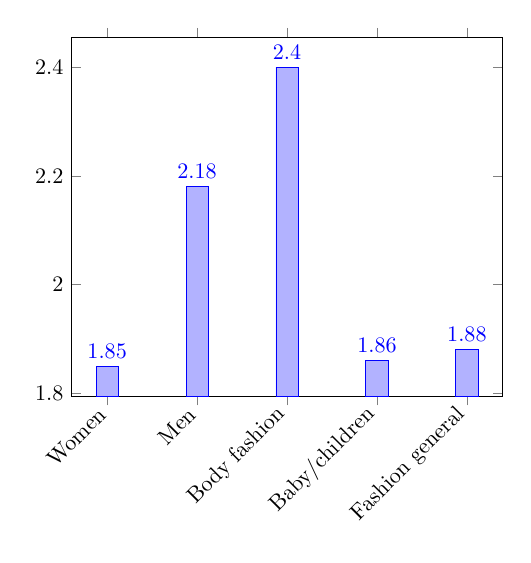
\begin{tikzpicture}[scale=0.8]
      \begin{axis}[
        ybar,
        symbolic x coords={Women, Men, Body fashion, Baby/children, Fashion general},
        x tick label style={rotate=45, anchor=east},
      ]
      \addplot +[nodes near coords] coordinates {
        (Women, 1.85)
        (Men, 2.18)
        (Body fashion, 2.40)
        (Baby/children, 1.86)
        (Fashion general, 1.88)
      };
      \end{axis}
    \end{tikzpicture}
    \caption{Conversion rate in various fashion segments}
    \label{fig:conversionRateFashion}
\end{figure}

This figure is taken from~\cite{Jorij2012} and shows the conversion rate for
various segments in the fashion domain. The conversion rate is the portion of
users who visits a website, and reaches the target (makes a conversion) set
by the site. For most e-commerce application, a conversion
is counted when a purchase is made. The conversion rate $r$ can easily be
calculated by $r = \frac{|Conversions|}{|Total visits|}$~\cite{nielsen2013}.
We can see that womens has the lowest conversion rate among the different
segments, indicating that there is a strong preference based shopping
tendency and that many users are \textit{browsing} and searching for the
right product. This hypothesis is strengthen by looking at the general
conversion rate in the e-commerce industry, which lies at 3\%. The potential
of a personalized recommender could in other words make browsing easier and
hence increase the conversion rate.

When making a purchase in the SoBazaar application, the user is redirected to the retailer selling the item, so the purchase is not done in the application.
This can lead to a higher \emph{purchase count} than the actual truth, but is what can be considered the conversion in the SoBazaar application.
For SoBazaar there are 18200 sessions in total and 1488 purchases, so the conversion rate is $0.08175824175 = \frac{1488}{18200}$, which is quite high compared to the conversion rate in women fashion from figure~\ref{fig:conversionRateFashion}, which was expected, since it is no commitment to making a purchase in the SoBazaar application.

\begin{figure}[H]
  \begin{tabular}{cc}
    \resizebox{0.43\linewidth}{!}{
      \begin{tikzpicture}
        \pie[text=legend, rotate=60]{
          34.30/Women,
          13.43/Men,
          17.91/Generalist,
          11.94/Body,
          4.47/Shoes,
          2.98/Jeans,
          14.97/Other
        }
      \end{tikzpicture}
    }
    \resizebox{0.49\linewidth}{!}{
      \begin{tikzpicture}
        \pie[text=legend, rotate=60]{
          15/Direct,
          23/Paid,
          30/Organic,
          5/CPS,
          9/CPC,
          8/Viral or social,
          10/E-mail newsletter
        }
      \end{tikzpicture}
    }
  \end{tabular}
  \caption{Distribution of target groups and traffic sources in the fashion
  domain}
\end{figure}

Both figures are adopted from~\cite{Jorij2012}, basing its results from a study
with 70 participating fashion companies with the goal of doing a complete
benchmark of the industry. In the leftmost figure we see how the different
e-commerce fashion retailers focuses their products. We observe that a large
majority of e-commerce fashion companies are targeting women - as is
SoBazaar.  Underlining the compensative market and the need to stand out to
the customer, by e.g. having personalized recommendations.

In the rightmost figure it is shown from where the customers originate in
online retails stores. The \textit{Paid} and \textit{Organic} are synonymous
with a user entering the site via. research or ads in the search engine, and
stands for 53\% of the traffic in e-commerce fashion - highlighting the
importance of a good reputation and digital profile. Direct traffic is as low
as 15\%, compared to the e-commerce industry in general where the same number
is 22.3\% \cite{Jorij2012}. This is explained by non-fashion products often
being offered in multiple stores and the users are thus browsing multiple sites
to find the best offer. Lastly we note that the viral/social segment is rather
small at 8\%, but compared to the e-commerce industry in general at 4\%. Hence
we conclude that although a small set of users interact with fashion companies
by social media, it is still a more important segment for this industry
compared to the e-commerce industry in general.

\subsection{Competitor Analysis}
\label{subsec:competitors}

As seen in the previous section, SoBazaar is not the only e-commerce
application in the fashion domain, with multiple competitors, and constantly new competitors entering the scene. Nor is it the first of its kind.

In this section some of these competitors will be explored,
looking into their strengths, weaknesses and features in regards to providing
recommendations for the user. This is both to better understand the fashion
domain (\textbf{Goal G1}) and to study existing technologies and how they are
applied (\textbf{Goal G3}). Using this data we can analyze the potential of
SoBazaar in e-commerce market, in addition we can understand both how users are
used to interact with similar applications and where we should focus in order
to enhance the uniqueness of the solution, creating a competitive advantage.

\subsubsection{Myntra}
\label{par:myntra}

"Myntra.com is a one stop shop for all your fashion and lifestyle needs" -
about Myntra~\cite{myntra}.

Myntra is one of India's largest e-commerce stores for fashion and aims to
provide a hassle free shopping experience for the user.  They aim to bring the
newest and most in-season fashion products available to the user trough the web
store front.  The brand base of Myntra consists of 500 leading brands from both
inside and outside India.

The web page uses a set of recommendation approaches to inform the user of what
they might like, and to increase the user's awareness of different kinds of
items. Such as, similar item and most popular. In this figure we can see in red
how Myntra is suggesting items which are similar to the item the user is
currently looking at

\begin{figure}[H]
    \centering
    \fbox{
      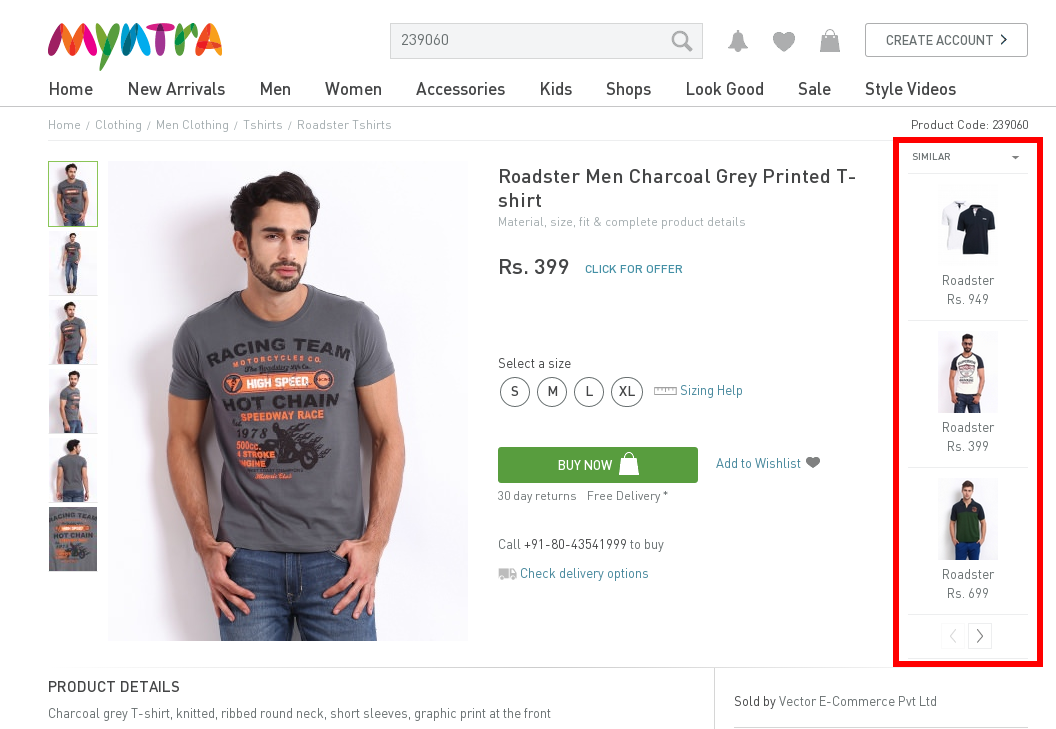
\includegraphics[scale=0.4]{image/myntiaSimilarExample.png}
    }
    \caption[Example of Myntra's "similar item" approach]{Example of Myntra's
    "similar item" approach}
    \label{figure:myntiaSimilarEx}
\end{figure}

This table is the list of the recommendation related strengths and weaknesses
of the e-commerce fashion web site Myntra~\cite{myntra}

\begin{table}[H]
    \centering
    \begin{tabularx}{\linewidth}{>{\parskip1ex}X@{\kern4\tabcolsep}>{\parskip1ex}X}
        \toprule
        \hfil\bfseries Strengths
        &
        \hfil\bfseries Weaknesses
        \\\cmidrule(r{3\tabcolsep}){1-1}\cmidrule(l{-\tabcolsep}){2-2}
        %Strengths
        Suggest similar items connected to the currently viewed \par
        Popular list for the different brands and stores \par
        Ability to add item to a "want list"\par
        &
        %Weaknesses
        No personalized recommendations \par
        \\\bottomrule
    \end{tabularx}
    \caption{Myntra: Strengths and weaknesses}
    \label{table:ecommerceMyntra}
\end{table}

\subsubsection{Asos}
\label{par:Asos}

"ASOS is a global online fashion and beauty retailer selling over 65,000 branded and own-label products" -
about Asos~\cite{asos}.

Asos have more than 29 million unique visitors per month and ship to more than 234 countries and territories.

The web page gives the user the ability to add products directly to a shopping chart.
When accessing an item, the user is presented with a set of items which asos recommends for the user.
They also present a set of clothes which might \emph{complete the look}, these recommendations are products which are assumed to \emph{go well} with the current item.
The users can also like and save items for later.
Other features are \emph{most popular} and \emph{outfits \& looks}.
\emph{Outfits \& looks} is a community where the user is given a set of options, amongst them are; voting for items, shop looks, gather \emph{style credits} and follow other users.

This table is the list of the recommendation related strengths and weaknesses
of the e-commerce fashion web site Asos~\cite{asos}

\begin{table}[H]
    \centering
    \begin{tabularx}{\linewidth}{>{\parskip1ex}X@{\kern4\tabcolsep}>{\parskip1ex}X}
        \toprule
        \hfil\bfseries Strengths
        &
        \hfil\bfseries Weaknesses
        \\\cmidrule(r{3\tabcolsep}){1-1}\cmidrule(l{-\tabcolsep}){2-2}
        %Strengths
        Suggest similar items connected to the currently viewed \par
        Popular list for the different brands and stores \par
        Ability to add item to a "want list" \par
        Suggest items which might \emph{go well} with other items \par
        Follow other users \par
        &
        %Weaknesses
        No personalized recommendations \par
        \\\bottomrule
    \end{tabularx}
    \caption{Asos: Strengths and weaknesses}
    \label{table:ecommerceAsos}
\end{table}


\subsubsection{Mallzee}
\label{par:Mallzee}

"Say hello to Mallzee, your nifty, personalised shopping app with a social twist. Instantly purchase, save for later or ask your nearest and dearest for their opinion on your latest fashion discovery." - about Mallzee~\cite{mallzee}.

Mallzee is a mobile phone application intended to ease shopping trough gathering fashion stores in one place, and have more than 2 million products from over 100 stores.

The applications utilizes a \emph{hot-or-not} approach, where the user can like or dislike products, this feedback is used to recommend other products the user might like.
Users can also get feedback from other users.

This table is the list of the recommendation related strengths and weaknesses
of the e-commerce fashion mobile application Mallzee~\cite{mallzee}

\begin{table}[H]
    \centering
    \begin{tabularx}{\linewidth}{>{\parskip1ex}X@{\kern4\tabcolsep}>{\parskip1ex}X}
        \toprule
        \hfil\bfseries Strengths
        &
        \hfil\bfseries Weaknesses
        \\\cmidrule(r{3\tabcolsep}){1-1}\cmidrule(l{-\tabcolsep}){2-2}
        %Strengths
        Presented with what friends like \par
        Ability to add item to a "want list" \par
        Follow other users \par
        Personalized recommendations \par
        Hot-or-Not approach \par
        &
        %Weaknesses
        No most popular list \par
        Redirected on purchase \par
        \\\bottomrule
    \end{tabularx}
    \caption{Mallzee: Strengths and weaknesses}
    \label{table:ecommerceMallzees}
\end{table}

\subsubsection{Lyst} % (fold)
\label{par:lyst}

"Lyst.com is a fashion shopping site that gives you your own shopping
experience, so you can discover more of the fashion you love" - About
Lyst~\cite{lyst}.

Lyst offers items from thousands of the leading brands and stores of the world.

The site allows the user to follow different stores or brands to receive the
latest items they have to offer.  The user is given a personalized "stylefeed",
which displays items from the different brands or stores the user is following.
It is also possible for the user to add items to the their profile.

On first login the user is presented with a set of brands and store the user
can like or dislike, to get the "stylefeed" started.  On access of an item, the
user is presented with related items, and the ability to add the item to a
collection.  When the user wants to buy an item, the site will redirect the
user to the store selling the item.

\begin{table}[H]
  \centering
    \begin{tabularx}{\linewidth}{>{\parskip1ex}X@{\kern4\tabcolsep}>{\parskip1ex}X}
    \toprule
      \hfil\bfseries Strengths
        &
        \hfil\bfseries Weaknesses
        \\\cmidrule(r{3\tabcolsep}){1-1}\cmidrule(l{-\tabcolsep}){2-2}
                Can follow brands and stores \par
                Connected with facebook \par
                Ability to add item to a "want list" \par
                "Stylfeed" based the user's follow list \par
                Show related items \par
                &
                Limited personalized recommendations \par
                \\\bottomrule
            \end{tabularx}
    \caption[Recommendation related strengths and weaknesses of Lyst~\cite{lyst}]{This table is the list of the recommendation related strengths and weaknesses of e-commerce fashion web site Lyst~\cite{lyst}}
    \label{table:ecommenreceLyst}
\end{table}

\subsubsection{Farfetch} % (fold)
\label{par:farfetch}

"farfetch.com forms the hub of a global fashion community that unites
independent boutiques around the world with fashion lovers" - About
Farfetch~\cite{Farfetch}

Farfetch is a collection of over 1000 boutiques from all over the world
gathered on one web page.  The user can shop directly on the page, and get the
item delivered to the doorstep with only one checkout process.

When browsing an item the user is presented with a set of recommendations
related to the current item, and previous browsing history.  The item can be
added to a "want list" or to the shopping chart.

\begin{figure}[H]
    \centering
    \fbox{
      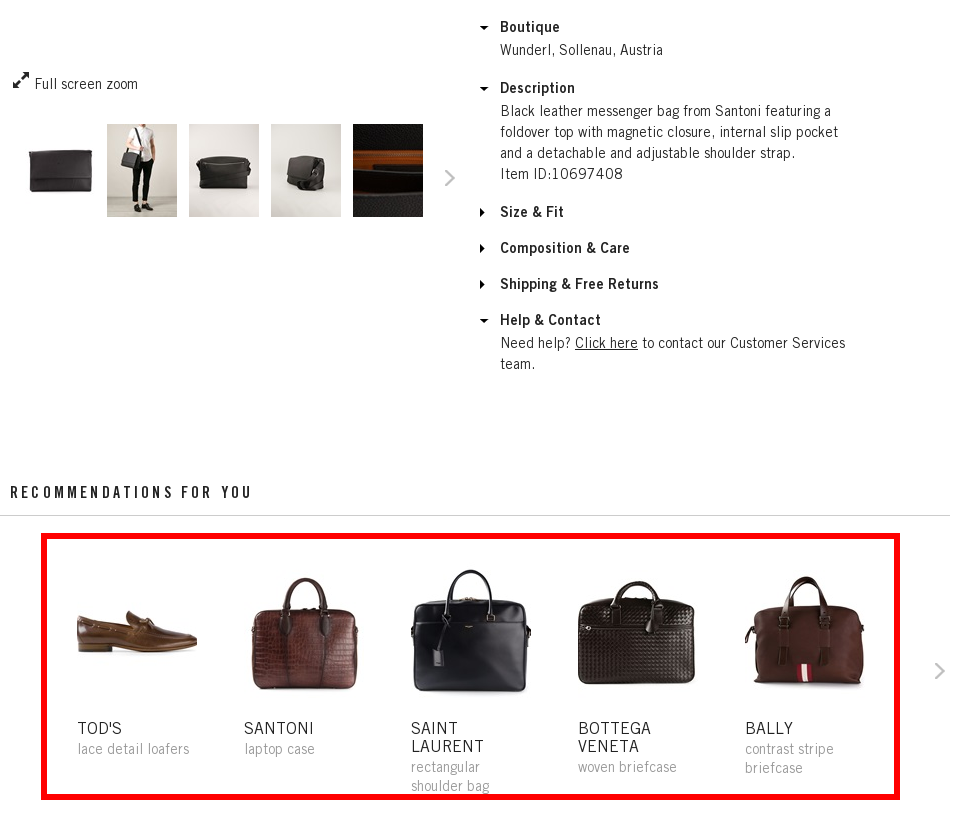
\includegraphics[scale=0.4]{image/farfetchedRecommendationExample.png}
    }
    \caption{Example of Farfetch's recommendations}
    \label{figure:farfetchedRecommendationExample}
\end{figure}

In this figure we can see in red how Farfetch is recommending items which might
be of interest to the user. As we can see the first item is a shoe, which was
the last item accessed by the user, the next four items are related to the
currently viewed item.

\begin{table}[H]
    \centering
    \begin{tabularx}{\linewidth}{>{\parskip1ex}X@{\kern4\tabcolsep}>{\parskip1ex}X}
      \toprule
      \hfil\bfseries Strengths
      &
      \hfil\bfseries Weaknesses
        \\\cmidrule(r{3\tabcolsep}){1-1}\cmidrule(l{-\tabcolsep}){2-2}
        %Strengths
            Ability to add item to a "want list" \par
            A feed with the most popular items \par
            A feed with new items \par
            A list of recommendations for the user \par
          &
          %Weaknesses
            No option to follow other users \par
         \\\bottomrule
    \end{tabularx}
    \caption[Recommendation related strengths and weaknesses of Farfetch~\cite{Farfetch}]{This table is the list of the recommendation related strengths and weaknesses of e-commerce fashion web site Farfetch~\cite{Farfetch}}
    \label{table:ecommenreceFarfetch}
\end{table}

\subsubsection{MyHabit}
\label{par:myhabit}

"MyHabit is a private fashion sale site offering up to 60\% off hand-picked
selections from designer and boutique brands." - About MyHabit~\cite{MyHabit}

MyHabit was founded by Amazon in response to the desire from the users of
Amazon to shop fashion in an easy manner.

The site displays a feed.  This feed is fed by a team from MyHabit, and is
constantly updating with new sales and new products.  The items put into the
feed are handpicked.

When browsing items on MyHabit, other similar items are suggested to the user.

\begin{table}[H]
  \centering
  \begin{tabularx}{\linewidth}{>{\parskip1ex}X@{\kern4\tabcolsep}>{\parskip1ex}X}
    \toprule
    \hfil\bfseries Strengths & \hfil\bfseries Weaknesses \\
    \cmidrule(r{3\tabcolsep}){1-1}\cmidrule(l{-\tabcolsep}){2-2}
    Shop on site \par
    Similar items \par
    &
    No personalized recommendations \par \\
    \bottomrule
  \end{tabularx}
  \caption[Recommendation related strengths and weaknesses of MyHabit~\cite{MyHabit}]{This table is the list of the recommendation related strengths and weaknesses of e-commerce fashion web site MyHabit~\cite{MyHabit}}
  \label{table:ecommenreceMyHabit}
\end{table}

\subsubsection{Competitors Recommendation Overview}
\label{par:competitors_recommendation_overview}

In table~\ref{table:ecommerceCommpetiros} we see that there is a very low count
of fashion related e-commerce applications, which actually produces
personalized recommendations for their users.

Most of applications are taking a simpler approach when making recommendations
for the user, like most popular or similar items.  There is no obvious relation
between recommendations and that the site has a form of "want list", but the
system which allows the users to follow each other are usually not
in-application-purchase-applications.

There where no indications of the "want list" being used directly to some
personalized recommendations and neither was it any indication that the "follow
list" of other users helped produce any personalized recommendations, other
than recommending items from the followed user's feed.  The "follow list" was
also in some cases used to suggest other users to follow.  The "want list" was
primarily there so that the user could go back to a liked item, and maybe
interact with it later.

\begin{table}[H]
    \centering
    \begin{tabular}{l l l l l l l}
        \toprule
        Competitor &
        \multicolumn{1}{l}{\parbox{1.3cm}{ In App \\ Purchase}} &
        \multicolumn{1}{l}{\parbox{1.0cm}{ Most \\ Popular}} &
        \multicolumn{1}{l}{\parbox{1.0cm}{ Similar \\ Items}} &
        \multicolumn{1}{l}{\parbox{1.0cm}{ Want \\ List}} &
        \multicolumn{1}{l}{\parbox{1.9cm}{ Follow \\ Other Users}} &
        \multicolumn{1}{l}{\parbox{2.6cm}{ Personalized \\ Recommendations}} \\ \midrule

        Myntra  & \cmark & \cmark & \cmark & \cmark & \xmark & \xmark \\
        Flink   & \xmark & \cmark & \cmark & \cmark & \cmark & \xmark \\
        Lyst    & \xmark & \cmark & \cmark & \cmark & \cmark & \xmark \\
        Motilo  & \xmark & \cmark & \xmark & \cmark & \cmark & \xmark \\
        Farfetch & \cmark & \cmark & \cmark & \cmark & \xmark & \xmark/\cmark~\tablefootnote{How the recommendations are produced is not mentioned} \\
        ModCloth  & \cmark & \cmark & \cmark & \cmark & \xmark & \xmark \\
        UsTrendy  & \cmark & \cmark & \cmark & \cmark & \xmark & \xmark \\
        Polyvore  & \xmark & \cmark & \cmark & \cmark & \cmark & \xmark \\
        Clothia  & \xmark & \cmark & \cmark & \cmark & \cmark & \xmark \\
        Trendabl  & \cmark & \cmark & \cmark & \cmark & \cmark & \xmark \\
        Zalando  & \cmark & \cmark & \cmark & \cmark & \xmark & \xmark \\
        Ellos  & \cmark & \cmark & \cmark & \cmark & \xmark & \xmark \\
        LookBook  & \xmark & \cmark & \cmark & \cmark & \cmark & \xmark \\
        Fahsiolista  & \xmark & \cmark & \xmark & \cmark & \cmark & \xmark \\
        ShopStyle  & \xmark & \xmark & \cmark & \cmark & \xmark & \xmark \\
        MyHabit  & \cmark & \xmark & \cmark & \xmark & \xmark & \xmark \\
        Asos  & \cmark & \cmark & \cmark & \cmark & \cmark & \xmark \\
        Mallzee  & \xmark & \xmark & \xmark & \cmark & \cmark & \cmark \\
        Kwoller  & \xmark & \xmark & \xmark & \cmark & \xmark & \cmark \\
        \bottomrule
    \end{tabular}
    \caption{Properties of different e-commerce application}
    \label{table:ecommerceCommpetiros}
\end{table}

Show in the table~\ref{table:ecommerceCommpetiros} above is the list of the
different properties of some of the different competitors to SoBazaar. The
properties are in regards of their recommendation ability, and how they let
their user expand their item set A more complete list can be found in the
appendix~\ref{app:sec:soCompetitors}.

\subsection{Fashion Recommender Systems}

This subsection will look at different methods other fashion related
systems have used to recommend fashion related products to the user.

\subsubsection{Photograph based approach}
    Fashion and the products it regards are highly dependent on visuals.  A fashion
    product would not be very interesting if no one saw it.  An approach to use the
    importance of how the product looks regarding recommending is to utilize images
    of the product.  Fashion Coordinates Recommender System Using Photographs from
    Fashion Magazines~\cite{Iwata:2011} is a system doing this.  They teach their
    system by using fashion magazines with full body images.  They segment the
    image into two parts, top and bottom.  From this the system learns which top
    matches to which bottom and collects visual features of the products.  From
    this the system can recommend other tops to go with a selected bottom, or other
    way around.  The proposed system scored better\footnote{Accuracy of 50\% on the
    top 5 suggested items, whereas naive and random managed 18\% and under 5\%
    respectively} than both a more naive approach and a random selection.  Runtime
    was at 0.04 seconds per recommendation.

\subsubsection{Hot-or-not}
    A recommender system called SuitUp~\cite{SuitUp} did a survey on some of their potential users.
    One interesting finding was that many of the users enjoyed the Hot-or-Not feature of the system.
    This feature gives the user a set of items and the option to either like or dislike.
    This did not only make the participants in the survey more engaged in the system, but also produced ratings, both negative and positive, for the system.
    For cold-start users and in a cold-start system this extra information and ratings make it much easier to make recommendations for the users.

\subsubsection{Scenario-Oriented Recommendation}
    Shen et al.~\cite{Shen:2007:AIG:1216295.1216368} proposed a recommender system which produce recommendations not only based on the metadata of the products, but also on user written input.
    Knowledge used to handle the user input, is derived from Open Mind Common Sense~\cite{Singh02openmind}.

    The user uploads his or her clothes and adds brand (e.g.Nike), type (e.g.jeans), material and a description about the item (e.g."I put these on when I get home").
    The systems makes recommendations based on the scenario the user is needing help to find suiting clothes to wear.
    The typical use case of the system is when a user is unsure about what to wear under different circumstances, but knows something about the scenario or occasion the clothes will be worn in.
    For instance: "I am going to the beach".
    It is also possible to interact with other users and the system relates similar users.

    The different describing fields about the items are given a six-tuple style value.
    The six tuples are: luxurious, formal, funky, elegant, trendy and sporty, where each is given a value from 0 to 10 based on how much the describing field of the items is the current tuple.
    The different describing fields are given a default value, which can be changed by the user if that this necessary. But it seems like this has to be done for all brands, material and type manually to initialize the system.

    This is an interesting approach to fashion and clothes recommendations but the need for user scenario input and a six-tuple description of the different describing fields, might not be desirable for the user or the system administrator in the long run.

    Yu-Chu et al.~\cite{Yu-Chu:2012:PCS:2376365.2376961} and Ying et al.~\cite{Ying2011} are other similar systems. Ying et al.~\cite{Ying2011} made a recommender based on the a similar concept, namely, what to wear in different situations.
    The system recommends two sets of top-to-toe clothing based on the current season, the occasion and the items the user has uploaded.
    The uploaded items must be given a set of descriptions, including the occasion to use the item.

    To recommend, the system uses the user profile of the user, which describes the interests of the user and the information given by the user about the different items in his or hers wardrobe.

\subsubsection{Photograph Recommendation Integrated with Occasion} % (fold)
    \label{par:photograph_recommendation_integrated_with_occasion}
    Liu et al.~\cite{Liu:2012:HMC:2393347.2393433} combined the two approaches from Iwata et al.~\cite{Iwata:2011} and Ying et al.~\cite{Ying2011} and Shen et al.~\cite{Shen:2007:AIG:1216295.1216368} and suggested a system which recommend clothes both based on the photographies and the occasion the clothes are to be worn.

    They do this by incorporating fashion rules like, what can you wear to which occasion, and what can you wear as a complete set to different occasions.
    The recommender learn the clothing recommendations through a latent support vector machine framework.
    They use this framework to match four potential functions: visual features vs. attribute, visual features vs. occasion, attributes vs. occasion and attribute vs. attribute.
    These are used together in a scoring function for clothing recommendation.

    Their system preformed better than the baselines, but was highly dependent on the human detection accuracy, since the learner was learning from fashion photographs.
% paragraph photograph_recommendation_integrated_with_occasion (end)
